\documentclass[a4paper]{article}
%\usepackage{inputenc}
\usepackage{csquotes}
\usepackage[margin=1.5cm]{geometry} % Change the margins
\usepackage[utf8]{inputenc} % - Defines what coding LaTeX uses. Use this one.
\usepackage[english]{babel}
\usepackage[T1]{fontenc}
\usepackage{graphicx} % - Package for including images in the document.
\usepackage{amsmath}
\usepackage{amssymb}
\usepackage{mathtools}
\usepackage{listings}
\usepackage{textgreek}
\usepackage{caption} % Correct spacing for captions
\usepackage{siunitx} % Package for handling numbers (ex \num{1e6}), units (ex \SI{15,3}{Nm}) and intervals (ex \SIrange{10}{20}{\celcius}) correctly
\sisetup{output-decimal-marker={,},range-phrase=--,range-units=single,exponent-product=\cdot} % If you write in English, remove output-marker...
\graphicspath{ {Images/} } % - Path to where the images are located on your computer. In this case I have a folder (look to the left) "Images" where the images are gathered.
\usepackage{hyperref} % - Package for including hyperlinks in the document.
\usepackage[style=apa,backend=biber]{biblatex} % APA-referenser
\usepackage{mhchem}
\DeclareLanguageMapping{swedish}{swedish-apa}  % APA-referenser
 % - Package for the bibliography ("referenser").
\addbibresource{references.bib} % - From where, i.e. which file, the references are taken. The bibliography file is called name.bib; see left column.

\title{MD5 Collision Attack}

\author{
Klas Mannberg \\
{klaman-8@student.ltu.se
} \\ \\

\includegraphics[width=0.2\textwidth]{ltu_swe.jpg}}
\date{10 September 2020}

\begin{document}

\maketitle


\tableofcontents


\section{Lab Tasks}
\subsection{Task 1: Generating Two Different Files with the Same MD5 Hash}
\textbf{Question 1:}

The output will have our prefix and $P/Q$, but no space inbetween. See image \ref{task1}.\\
\textbf{Question 2:}


Having a prefix of exactly 64 bytes seems to add an empty region between our input and $P/Q$. See image \ref{question2}. Since it is already past 64 bytes when it adds the length, it is forced to add additional 64 space.\\
\textbf{Question 3: }

The last bytes of the output, $P/Q$, have a few differences. All other data is the same. \\
\subsection{Task 2: Understanding MD5’s Property}
If we know that the MD5 hash is the same with inputs $M$ and $N$, then adding a suffix $T$ to both will make the new files share the same md5 hash.
To show this I run the collision generator on a prefix of 64 bytes, which will generate $MD5(M)\:=\:MD5(N)$. In theory adding the same data $T$ to both with $cat$ will gives us $MD5(M || T) = MD5(N || T)$. This is what we do in image \ref{task2}. I add the file "suffix" to the end of both output files. The suffix file just contains the string \textit{BBBBBBBBBBB} in hex. The files having the same MD5 hash confirms the property.
\subsection{Task 3: Generating Two Executable Files with the Same MD5 Hash} \label{section:3}
The prefix ranges need to be in multiple of 64. Using bless I can find the array location which allows me to calculate the byte range from the start of the file $prefix$, or the bottom $suffix$. The closest prefix range which allowed the prefix to be divisible by 64, and be within the array, was $4224$. We know the prefix is $4224$ and that $P/Q$ will add 128 bytes, so the suffix must be the only remaining bytes of the file $\implies tail -c +4289\:a.out > suffix$.

After by running md5collgen on the prefix to get $P/Q$ added, we appended the suffix to both output files. The result is two executables with same md5 hash and different array values, see image \ref{task3_big}.
\subsection{Task 4: Making the Two Programs Behave Differently}
The goal here is to create a program with code that only triggers when a difference in data is detected. From Task 3 we know that we can make a program have different data, with the same MD5 hash. Using arrays we can leave a section of code that only triggers when it detects a difference between them. See image \ref{task4_code} for the code.\\

Since the prefix is 4160 (bytes to the start of the array) we do $head\:-c\:4160\:a.out\:>\:prefix$ and the suffix is the bytes after the 128 byte region $\implies tail\:-c\:+4289\:a.out > suffix$.
After cutting out the 128 bytes for P and Q from the output of $md5collgen$ we could now have two programs with different arrays. But it's a bit more compilcated since if we only change one of the arrays then the condition in our code will trigger for both programs (since $P$ is different from the A's in the array). The solution to this is to cut another 288 bytes, the distance to start of the second array, and insert $P$ there aswell. 
The only remaining part we need to cut out is the last bytes of the suffix after $P$ in the second array, which is \textit{Suffix3} in the example below.

Patching all this together we get:
\begin{enumerate}
  \item done1 = Prefix + P + Suffix2 + P + Suffix3
  \item done2 = Prefix + Q + Suffix2 + P + Suffix3 \\ \\
  \textit{Suffix2 is the space between the end of 128 byte $P$ or $Q$ in one array and the start of $P$ in the second} \\
  \textit{Suffix3 is the last bytes of suffix after second $P$}
\end{enumerate}

So now our hidden code only triggers on the program "done2" while both has the same MD5 hash. See image \ref{task4} for the result of $md5sum$. \\

Done1 will send you a nice message while done2 will curse your directory with 10 useless files! How terribly evil, I know.
\newpage
\section{Images}
\
\begin{figure}
  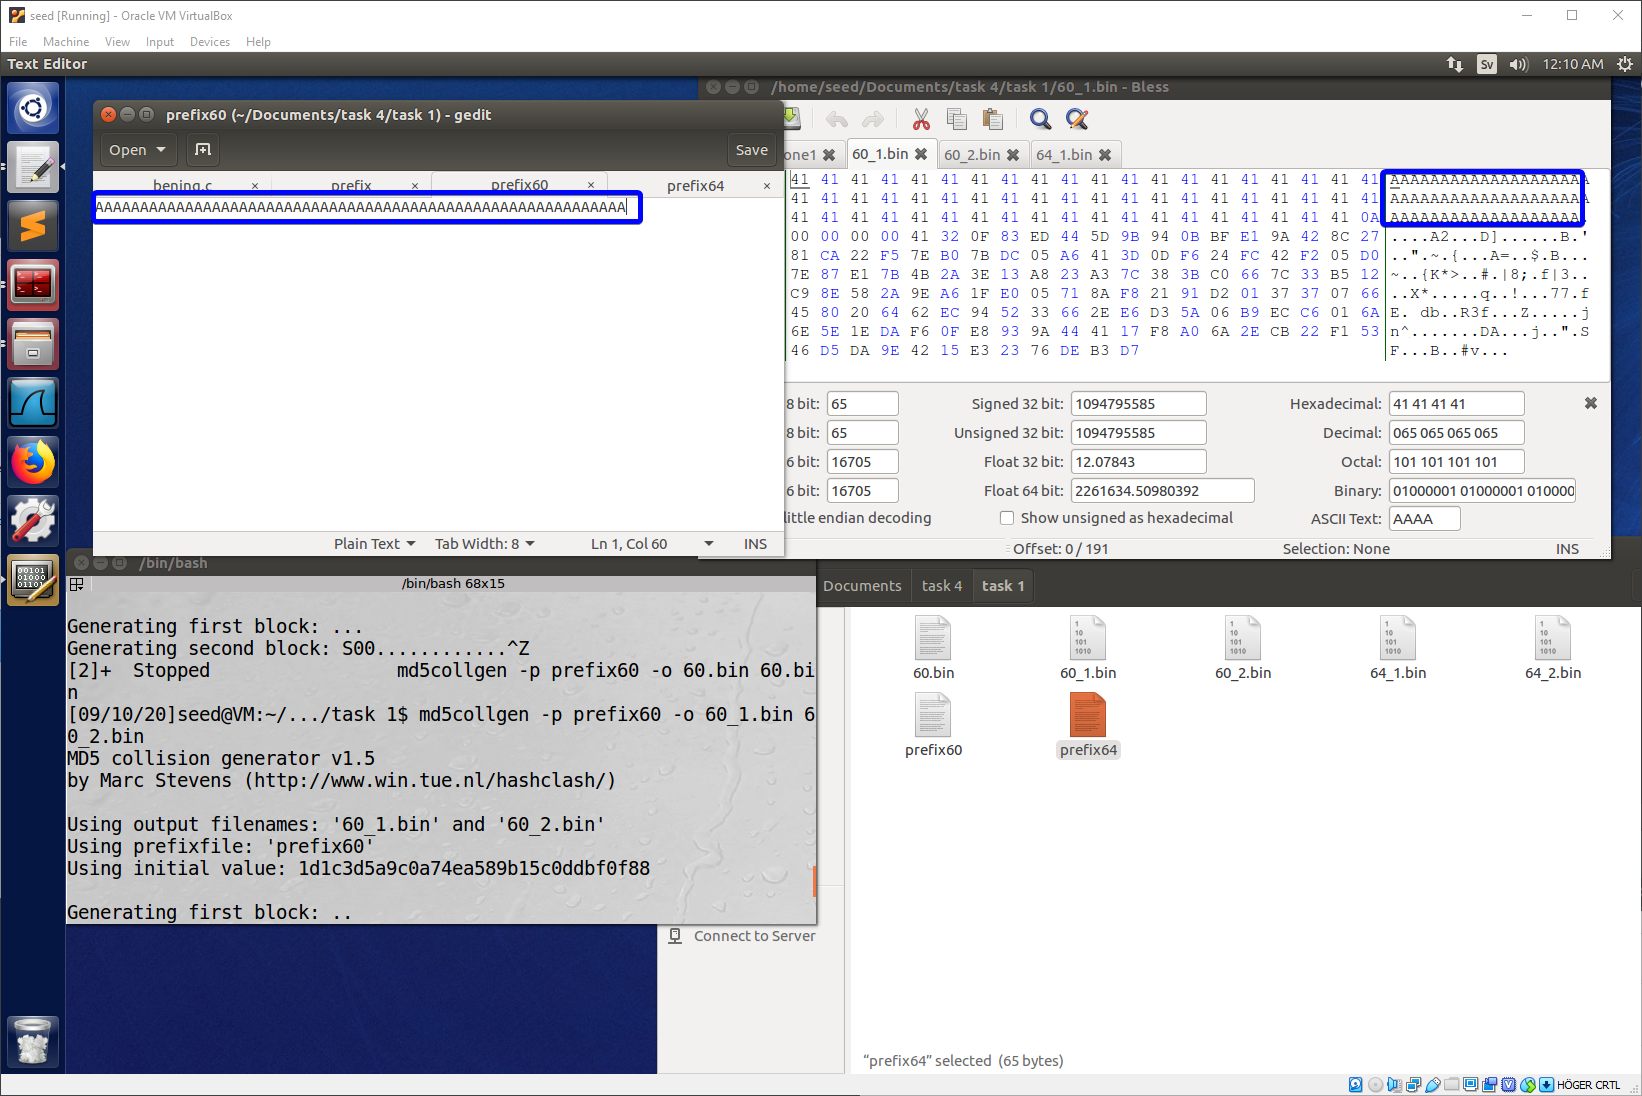
\includegraphics[width=\textwidth]{task1.png}
  \caption{Task 1, Question 1: Prefix and $P/Q$}
  \label{task1}
\end{figure}
\begin{figure}
  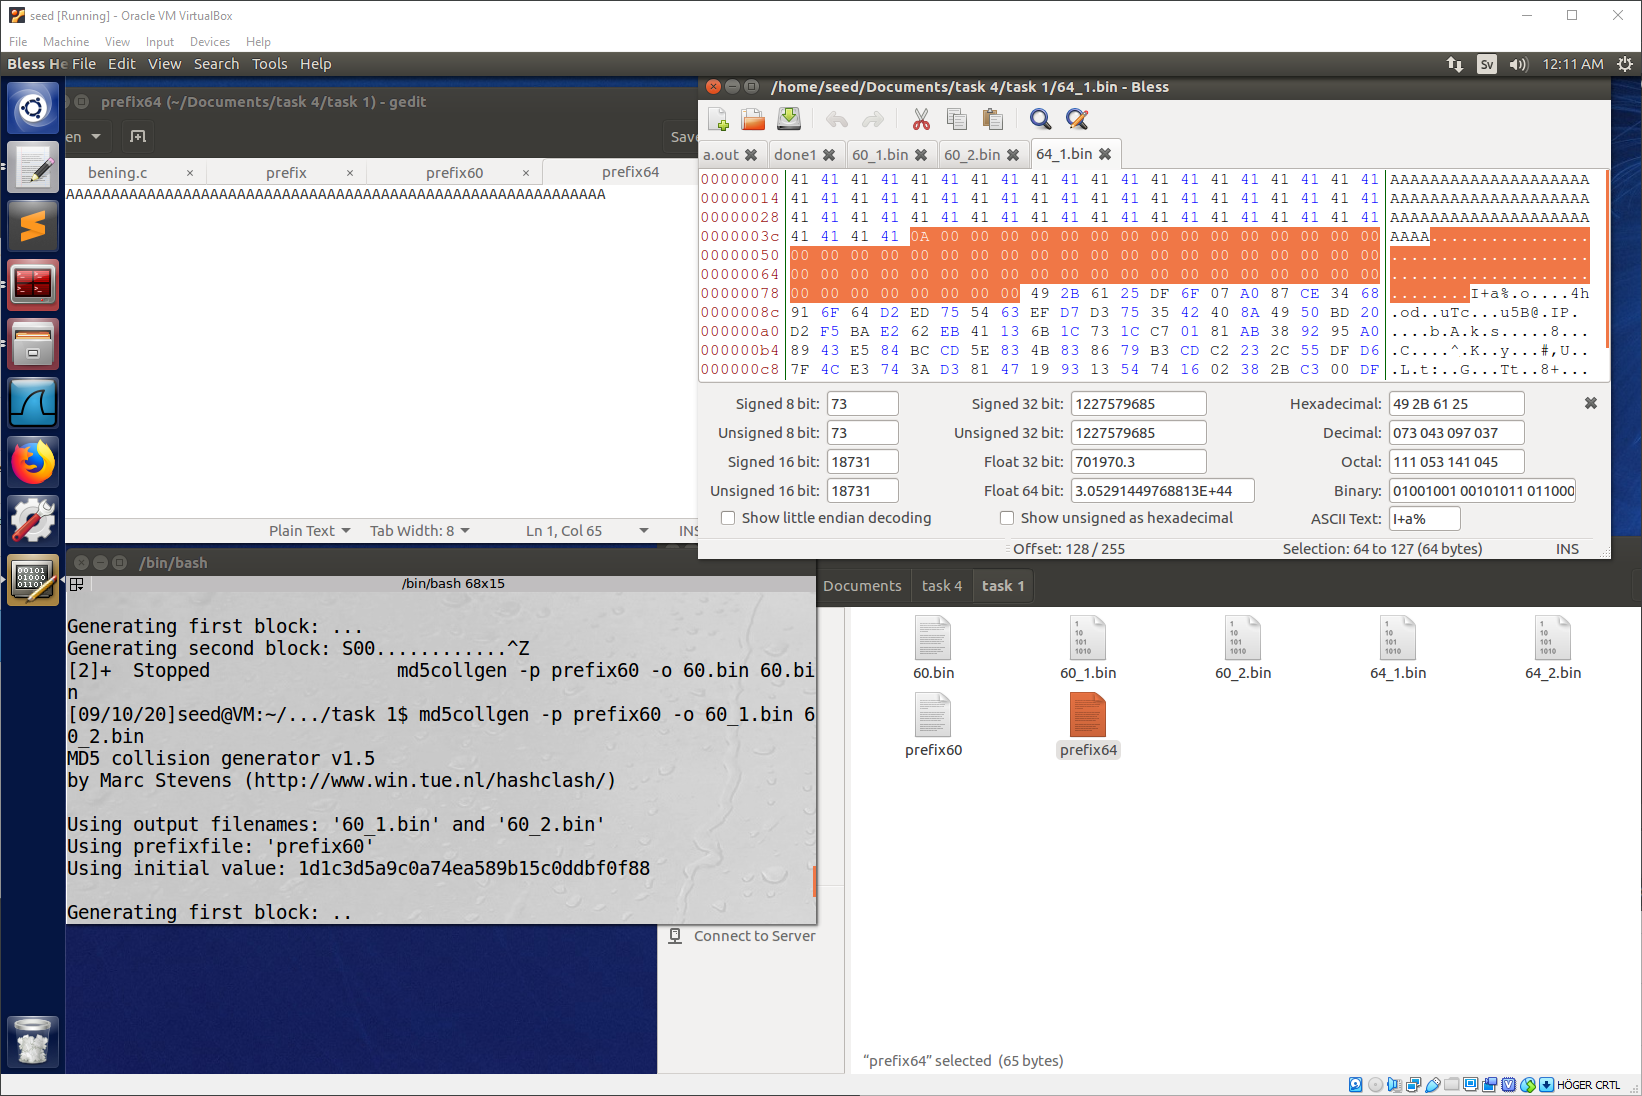
\includegraphics[width=\textwidth]{question2.png}
  \caption{Task 1, Question 2: Empty region}
  \label{question2}
\end{figure}
\begin{figure}
  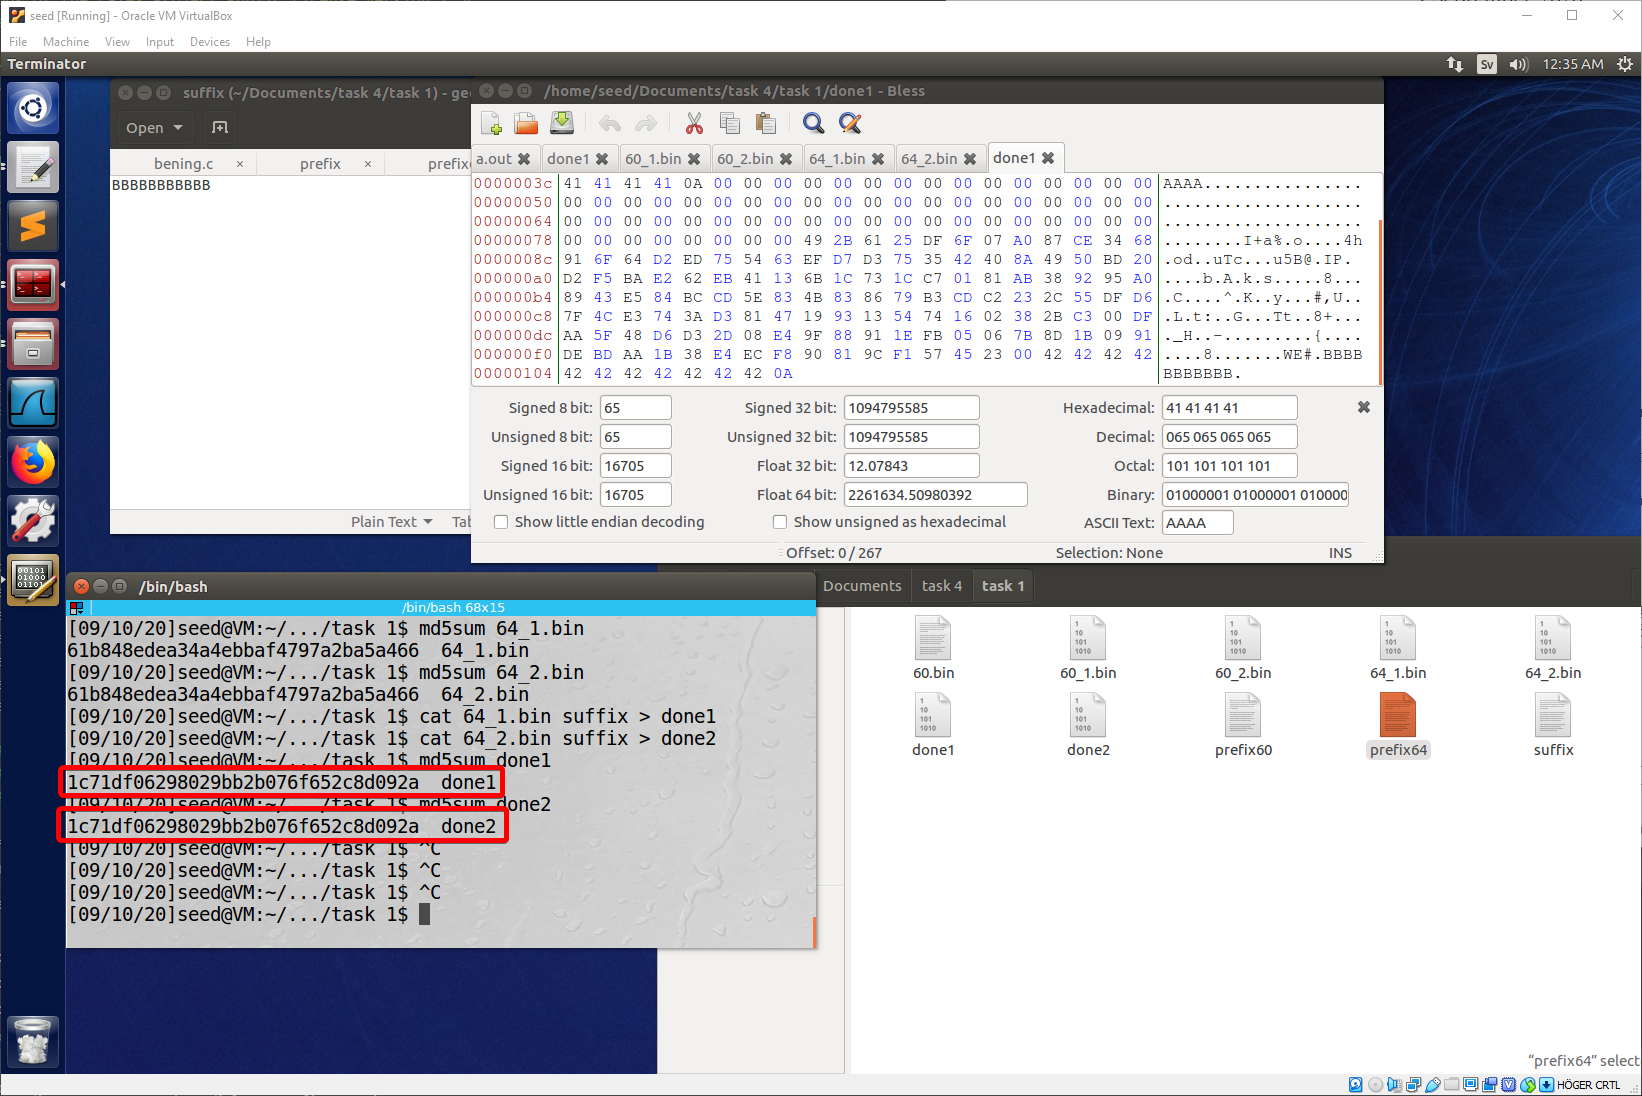
\includegraphics[width=\textwidth]{task2.png}
  \caption{Adding the suffix, $T$ "BBBBBBBBBBB" to the outputs $64_1.bin$ and $64_2.bin$ of the collision generator. Results have the same MD5 Hash}
  \label{task2}
\end{figure}
\begin{figure}
  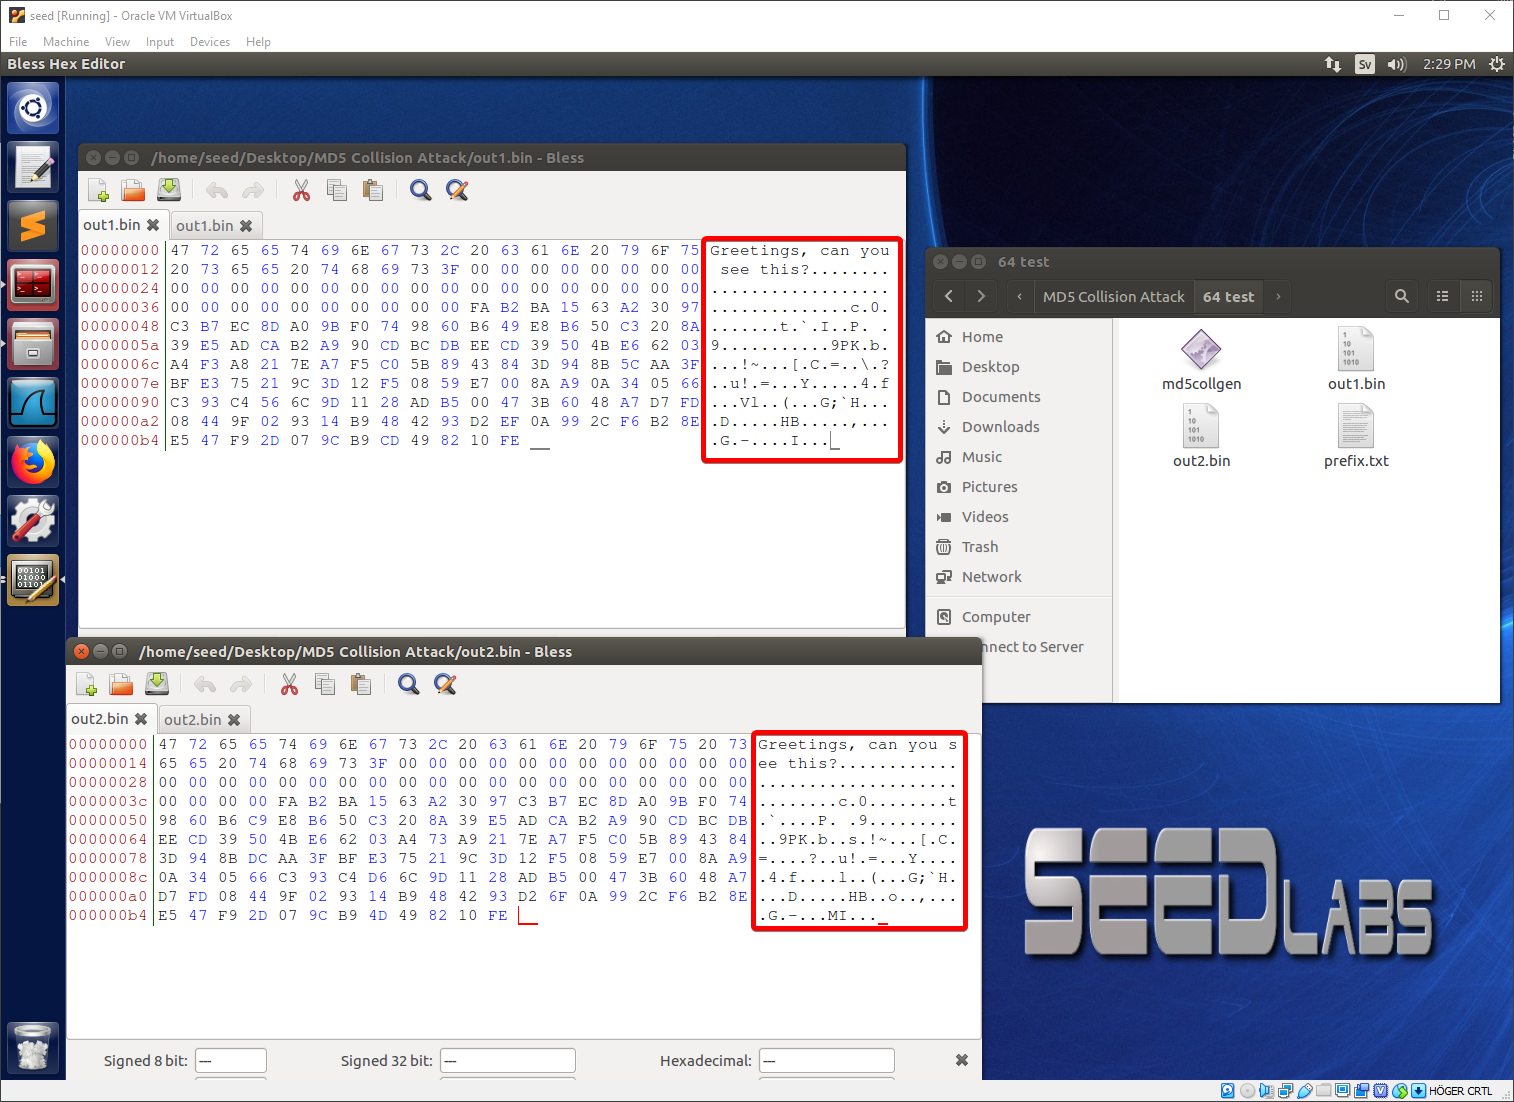
\includegraphics[width=\textwidth]{task1_2.png}
  \caption{The prefix+padding+generated contents of the bin files}
\end{figure}
\begin{figure}
  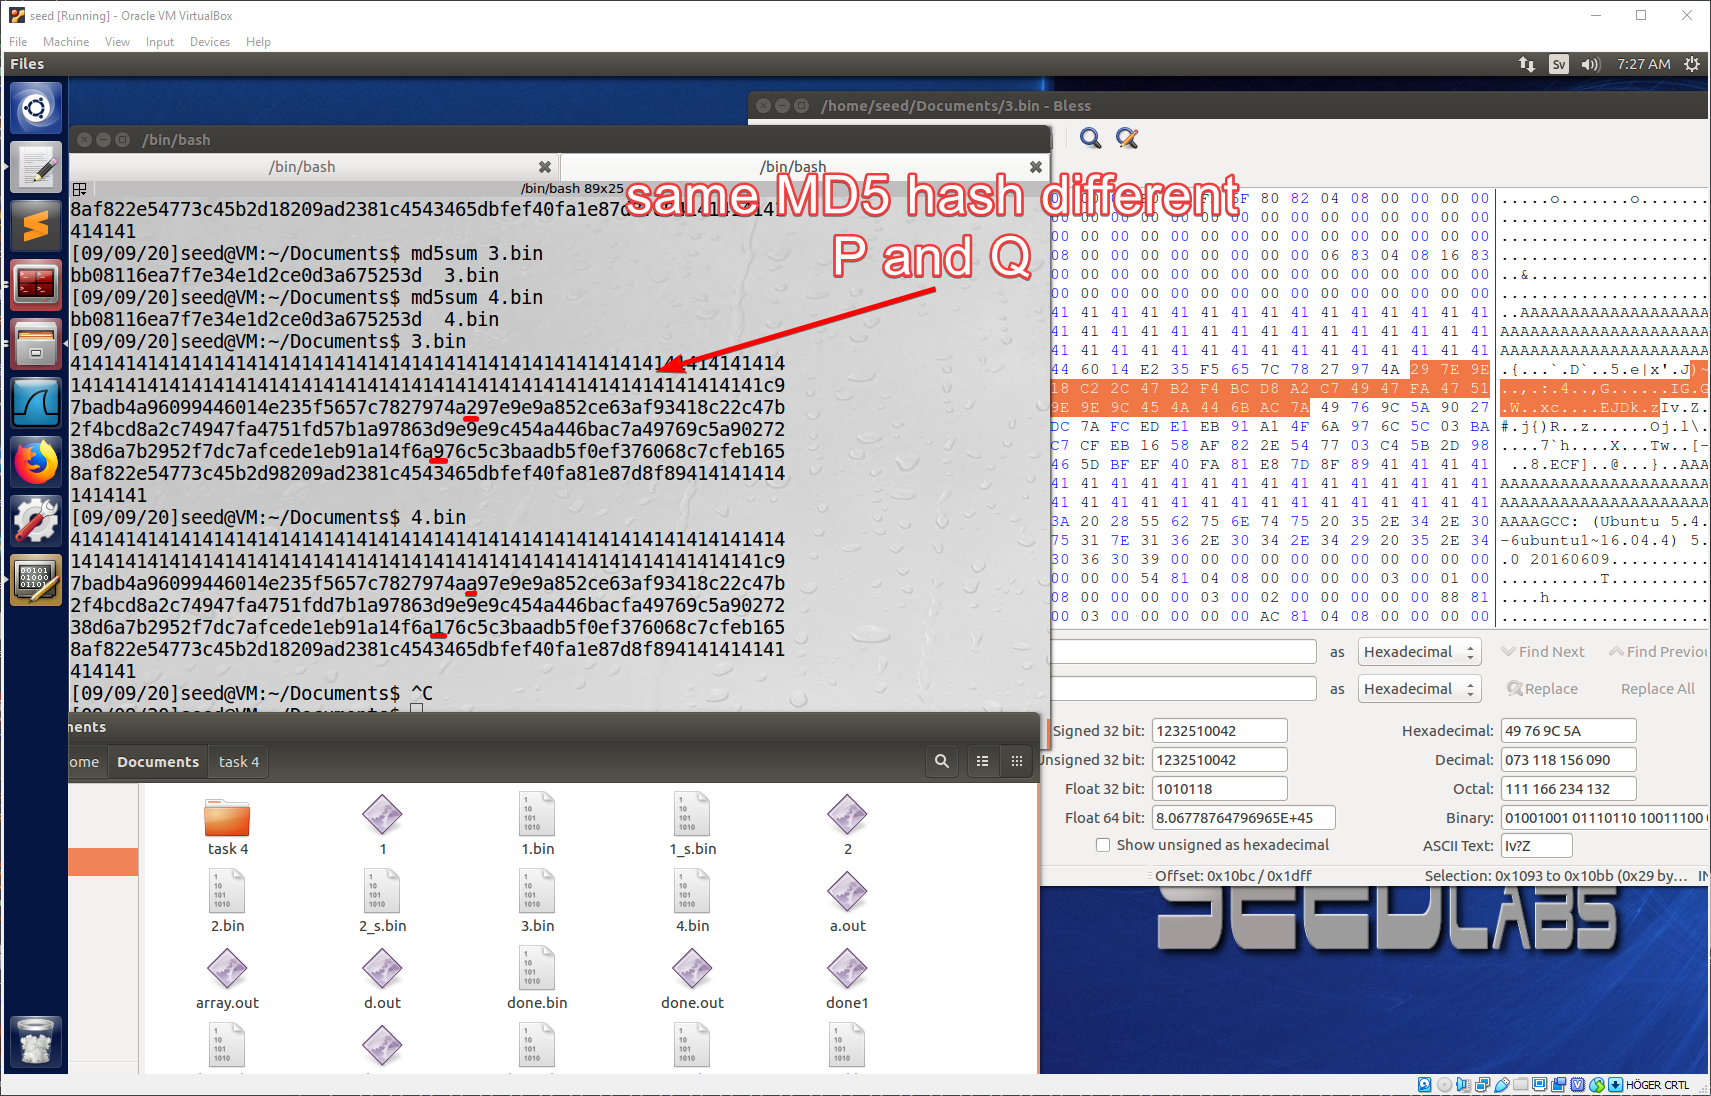
\includegraphics[width=\textwidth]{task3_big.png}
  \caption{Same MD5 hash but modified array!}
  \label{task3_big}
\end{figure}
\begin{figure}
  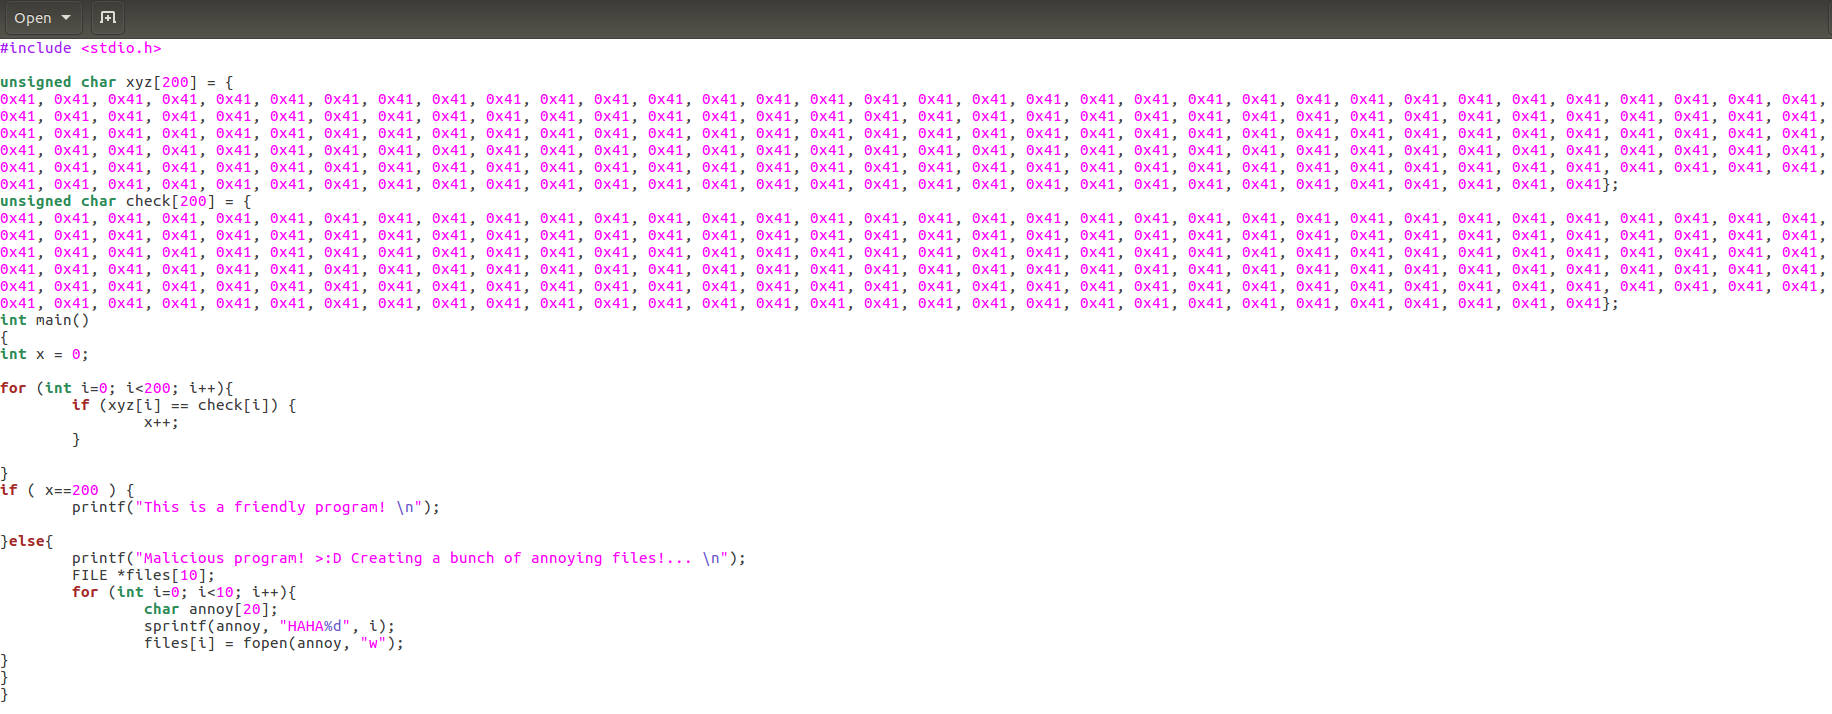
\includegraphics[width=\textwidth]{task4_code.png}
  \caption{Source code of task 4}
  \label{task4_code}
\end{figure}
\begin{figure}
  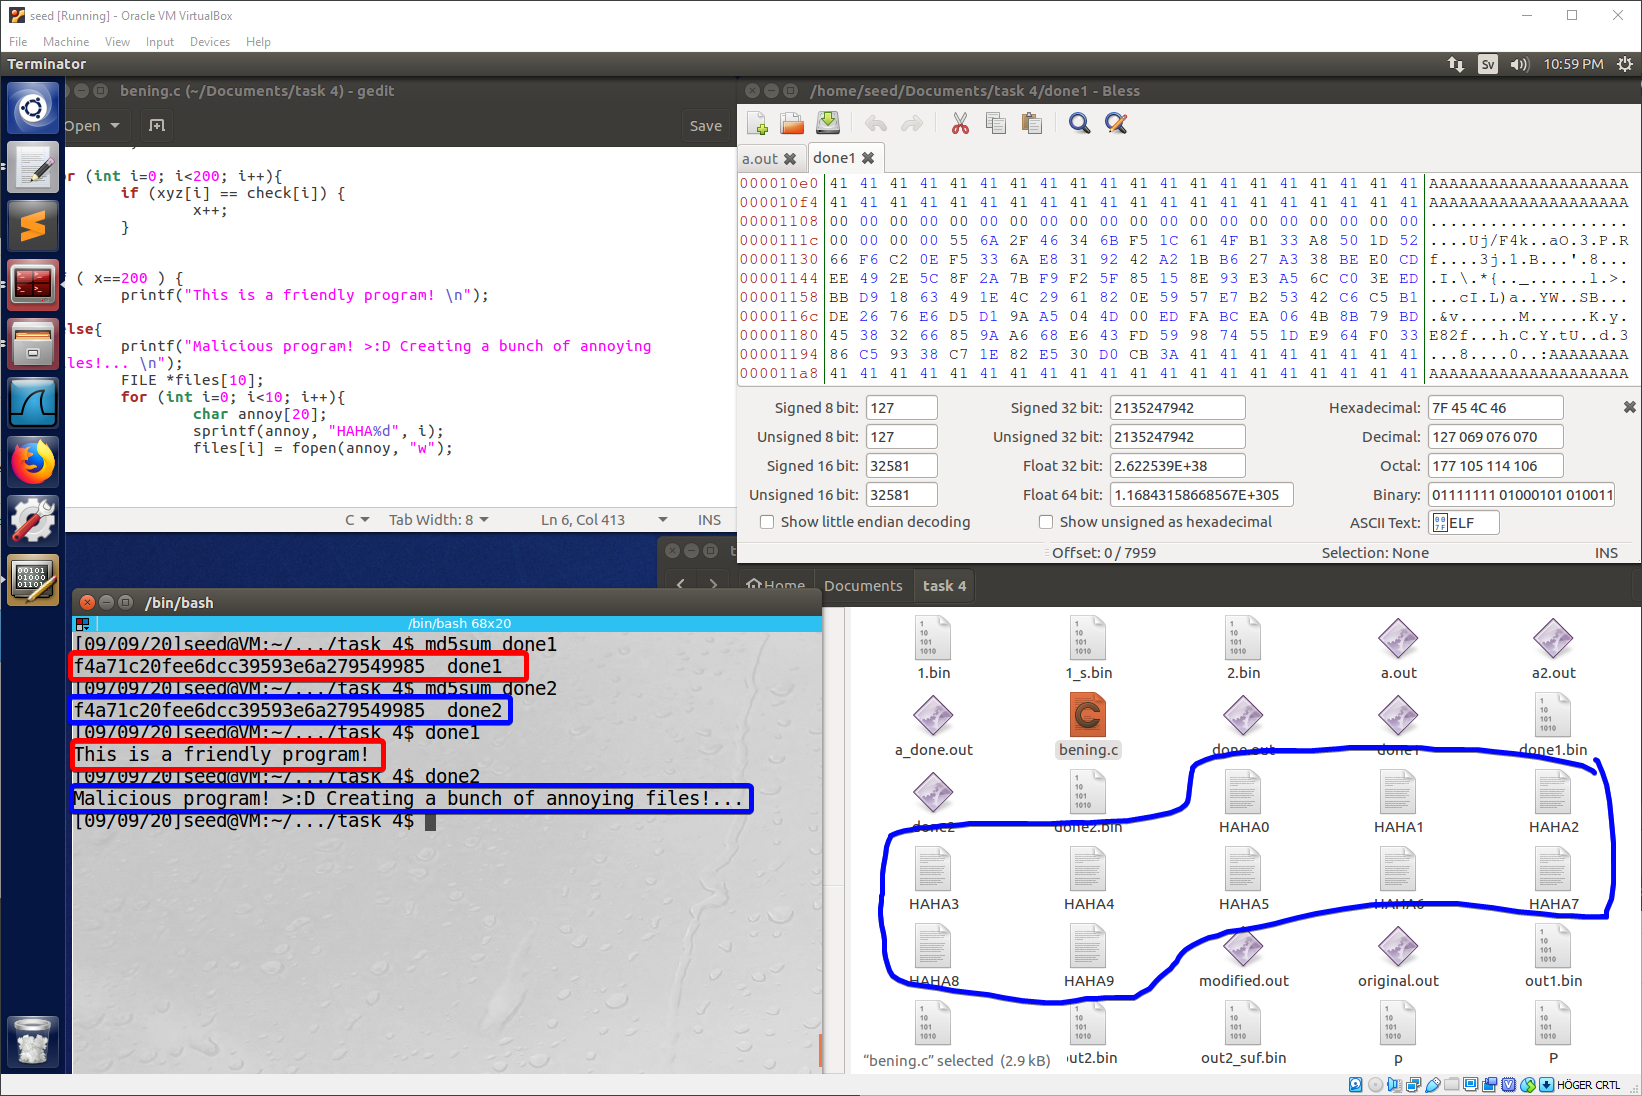
\includegraphics[width=\textwidth]{task4.png}
  \caption{Task 4: Two different sections of code executing, with same MD5 hash!}
  \label{task4}
\end{figure}

\end{document}
